% ==============================================================================
%  3.5  ANOVA en regresión simple. Descomposición de la variabilidad
%  3.6  El contraste de la regresión. F-test general
% ==============================================================================
\section{ANOVA en regresión simple}
\label{sec:t3-anova}

El análisis de regresión puede abordarse desde la perspectiva del \textbf{análisis de la
varianza (ANOVA)}, que se basa en la descomposición de la variabilidad de la respuesta $Y$. La
variabilidad se mide mediante las desviaciones de cada observación respecto de su media,
$Y_i-\media{Y}$, que se descomponen en
\[
  Y_i-\media{Y} = (Y_i-\est{Y}_i) + (\est{Y}_i-\media{Y}) .
\]

\begin{figure}[H]
  \centering
  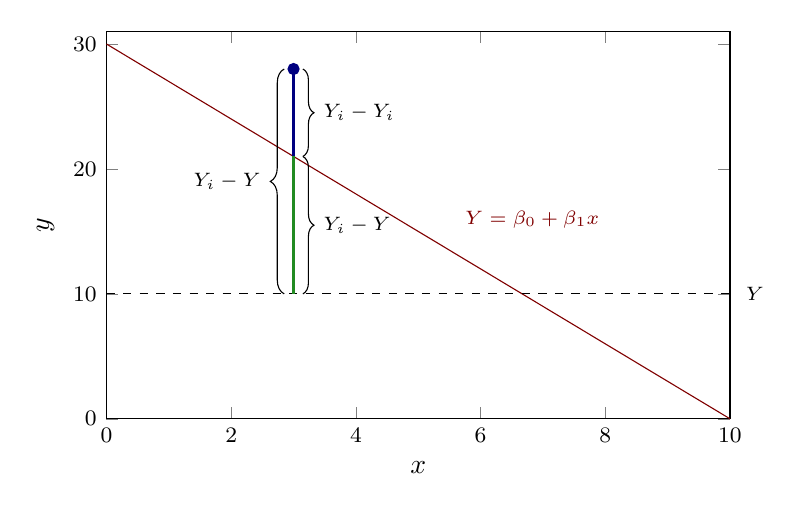
\begin{tikzpicture}
    \begin{axis}[width=9.5cm, height=6.5cm, xmin=0, xmax=10, ymin=0, ymax=31,
        xlabel={$x$}, ylabel={$y$}, tick label style={font=\footnotesize}, clip=false]
      \addplot[Maroon, no marks, domain=0:10] {30-3*x};
      \addplot[black, dashed, no marks, domain=0:10] {10};
      \node[font=\scriptsize, anchor=west] at (axis cs:10.1,10) {$\media{Y}$};
      \node[font=\scriptsize, Maroon, anchor=south west] at (axis cs:5.6,14.5) {$\est{Y}=\est{\beta}_0+\est{\beta}_1x$};
      \addplot[only marks, mark=*, mark size=2pt, NavyBlue] coordinates {(3,28)};
      \draw[NavyBlue, thick] (axis cs:3,28) -- (axis cs:3,21);
      \draw[ForestGreen, thick] (axis cs:3,21) -- (axis cs:3,10);
      \draw[decorate, decoration={brace, amplitude=4pt}] (axis cs:3.15,28) -- (axis cs:3.15,21)
        node[midway, right=4pt, font=\scriptsize] {$Y_i-\est{Y}_i$};
      \draw[decorate, decoration={brace, amplitude=4pt}] (axis cs:3.15,21) -- (axis cs:3.15,10)
        node[midway, right=4pt, font=\scriptsize] {$\est{Y}_i-\media{Y}$};
      \draw[decorate, decoration={brace, amplitude=5pt, mirror}] (axis cs:2.85,28) -- (axis cs:2.85,10)
        node[midway, left=5pt, font=\scriptsize] {$Y_i-\media{Y}$};
    \end{axis}
  \end{tikzpicture}
  \caption{Descomposición de la desviación de una observación respecto de la media.}
\end{figure}

\begin{teorema}[Descomposición de la variabilidad][teo:t3-sst]
  \[
    \underbrace{\sumi (Y_i-\media{Y})^2}_{SST}
    = \underbrace{\sumi (\est{Y}_i-\media{Y})^2}_{SSR}
    + \underbrace{\sumi (Y_i-\est{Y}_i)^2}_{SSE},
  \]
  es decir, variabilidad total de $Y$ = variabilidad explicada por la regresión + variabilidad no
  explicada por la regresión.
\end{teorema}

\begin{demostracion}
  Elevando al cuadrado $Y_i-\media{Y}=(Y_i-\est{Y}_i)+(\est{Y}_i-\media{Y})$ y sumando,
  \[
    SST = SSE + SSR + 2\sumi e_i(\est{Y}_i-\media{Y}),
  \]
  con $e_i=Y_i-\est{Y}_i$. Por las propiedades 1 y 5 de la recta de regresión
  (\cref{prop:t2-propiedades-recta}), $\sum e_i=0$ y $\sum\est{Y}_ie_i=0$, luego
  \(
    \sumi e_i(\est{Y}_i-\media{Y}) = \sumi \est{Y}_ie_i - \media{Y}\sumi e_i = 0 .
  \)
\end{demostracion}

\subsection{Los tres componentes}

\paragraph{Variabilidad total, $SST=\sum(Y_i-\media{Y})^2$.} Sin tener en cuenta $X$, el mejor
predictor de $Y$ es $\media{Y}$, y $SST$ es la suma de las desviaciones cuadráticas respecto de
él. Tiene $n-1$ grados de libertad, ya que hay que estimar $\media{Y}$ (equivalentemente, las
desviaciones $Y_i-\media{Y}$ suman 0). La media cuadrática $MST=SST/(n-1)$ es el estimador
habitual de la varianza cuando no hay ningún predictor.

\paragraph{Variabilidad explicada por el modelo, $SSR=\sum(\est{Y}_i-\media{Y})^2$.}
\begin{itemize}
  \item $\est{Y}_i-\media{Y}$ son las desviaciones de la recta ajustada (que tiene en cuenta $X$)
    respecto del mejor predictor sin tener en cuenta $X$.
  \item Si no hay relación entre $X$ e $Y$ ($\est{\beta}_1=0$), entonces
    $\est{Y}_i=\est{\beta}_0=\media{Y}$ para todo $i$ y $SSR=0$. En otro caso, $SSR>0$.
  \item Tiene \textbf{1 grado de libertad}: aunque hay $n$ desviaciones, todos los $\est{Y}_i$ se
    calculan con la misma recta, con 2 grados de libertad (\emph{intercept} y pendiente), y se pierde
    uno porque las desviaciones $\est{Y}_i-\media{Y}$ suman 0. La media cuadrática es $MSR=SSR/1$.
\end{itemize}

\paragraph{Variabilidad no explicada o residual, $SSE=\sum(Y_i-\est{Y}_i)^2$.}
\begin{itemize}
  \item Al usar $X$ como predictor, la variabilidad queda representada por las desviaciones de
    cada observación a la recta ajustada, $Y_i-\est{Y}_i$.
  \item $SSE=0$ si todas las observaciones coinciden con sus valores ajustados, y es mayor
    cuanto mayor es la dispersión alrededor de la recta.
  \item Tiene $n-2$ grados de libertad, ya que hay que estimar los dos coeficientes para calcular
    los $\est{Y}_i$. La media cuadrática $MSE=SSE/(n-2)$ es la mejor estimación de la varianza de
    $Y$ una vez que se condiciona a la variable explicativa.
\end{itemize}
Los grados de libertad también se descomponen: $n-1 = 1 + (n-2)$.

\subsection{El contraste de la regresión}

Las medias cuadráticas son variables aleatorias, puesto que lo son las $Y_i$. Sus esperanzas son
\[
  \E(MSE) = \sigma^2, \qquad \E(MSR) = \sigma^2 + \beta_1^2\,\SSX .
\]
Por tanto:
\begin{itemize}
  \item $MSE$ es un estimador insesgado de $\sigma^2$;
  \item si $\beta_1=0$ (no hay relación lineal), $MSR$ también es un estimador insesgado de
    $\sigma^2$;
  \item si $\beta_1\neq0$, $\E(MSR)>\E(MSE)$, ya que $\beta_1^2\SSX>0$.
\end{itemize}
Esto sugiere usar el cociente $MSR/MSE$ para contrastar $\beta_1=0$: cuanto mayor sea, más
evidencia habrá en contra de $\beta_1=0$.

\paragraph{Distribución bajo $H_0\colon\beta_1=0$.}
\begin{itemize}
  \item Si las $Y_i$ son independientes y proceden de la misma normal con varianza $\sigma^2$,
    $SST$ es una suma de cuadrados con $n-1$ grados de libertad y $SST/\sigma^2\sim\chisq{n-1}$.
  \item $SST$ es la suma de $SSR$ y $SSE$, cuyos grados de libertad, 1 y $n-2$, suman $n-1$.
  \item Si $\beta_1=0$, todas las $Y_i$ tienen la misma media $\beta_0$ y la misma varianza
    $\sigma^2$, y $SSR/\sigma^2$ y $SSE/\sigma^2$ son variables independientes con distribuciones
    $\chisq{1}$ y $\chisq{n-2}$, respectivamente.
\end{itemize}
En consecuencia,
\[
  F = \frac{MSR}{MSE} = \frac{\dfrac{SSR}{\sigma^2}\Big/1}{\dfrac{SSE}{\sigma^2}\Big/(n-2)}
  = \frac{\chisq{1}/1}{\chisq{n-2}/(n-2)} \bajoHo \Fdist{1}{n-2} .
\]

\begin{resumen}[Contraste de la regresión (F-test)]
  Para $H_0\colon\beta_1=0$ frente a $H_1\colon\beta_1\neq0$, con $F^*$ el valor observado de
  $F=MSR/MSE$:
  \begin{itemize}
    \item si $F^*\le\Fq{1}{n-2}{1-\alpha}$, no se rechaza $H_0$ a nivel $\alpha$;
    \item si $F^*>\Fq{1}{n-2}{1-\alpha}$, se rechaza $H_0$ a nivel $\alpha$.
  \end{itemize}
  En la práctica, se rechaza $H_0$ si el $p$-valor es menor que $\alpha$.
\end{resumen}

\paragraph{Equivalencia con el contraste $t$.} Para un nivel $\alpha$ dado, el test $F$ es
equivalente al \textbf{test bilateral} basado en la $t$ de Student para $H_0\colon\beta_1=0$. En
efecto, como $\est{\beta}_0=\media{Y}-\est{\beta}_1\media{X}$,
\[
  \est{Y}_i-\media{Y} = \est{\beta}_0+\est{\beta}_1x_i-\media{Y} = \est{\beta}_1(x_i-\media{X})
  \quad\Longrightarrow\quad
  SSR = \est{\beta}_1^2\sumi (x_i-\media{X})^2 = \est{\beta}_1^2\,\SSX ,
\]
y, puesto que $\widehat{\Var}(\est{\beta}_1)=MSE/\SSX$,
\[
  F = \frac{MSR}{MSE} = \frac{\est{\beta}_1^2\,\SSX}{MSE}
  = \frac{\est{\beta}_1^2}{\widehat{\Var}(\est{\beta}_1)}
  = \left(\frac{\est{\beta}_1}{\sqrt{\widehat{\Var}(\est{\beta}_1)}}\right)^2 = (t^*)^2 ,
\]
el cuadrado del estadístico $t$. La equivalencia es solo con el contraste \emph{bilateral}.

\subsection{La tabla ANOVA}

Toda la información anterior se resume en la \textbf{tabla ANOVA}:
\begin{center}
  \renewcommand{\arraystretch}{1.3}
  \begin{tabular}{lccccc}
    \toprule
    Fuente & $SS$ & g.l. & $MS$ & $F$ & $p$-valor \\
    \midrule
    Modelo (regresión) & $SSR$ & $1$ & $MSR$ & $F^*=MSR/MSE$ & $p$ \\
    Error & $SSE$ & $n-2$ & $MSE$ & & \\
    Total & $SST$ & $n-1$ & & & \\
    \bottomrule
  \end{tabular}
\end{center}

\begin{ejemplo}[Volumen de madera: tabla ANOVA][ej:t3-anova-arboles]
  \begin{center}
    \renewcommand{\arraystretch}{1.2}
    \begin{tabular}{lrrrrr}
      \toprule
      Fuente & $SS$ & g.l. & $MS$ & $F$ & $p$-valor \\
      \midrule
      Modelo & 3085.789 & 1 & 3085.789 & 84.34 & $<0.0001$ \\
      Error & 658.570 & 18 & 36.587 & & \\
      Total & 3744.358 & 19 & & & \\
      \bottomrule
    \end{tabular}
  \end{center}
  La salida del programa (SAS) incluye además los siguientes estadísticos:
  \begin{center}
    \renewcommand{\arraystretch}{1.2}
    \begin{tabular}{lr@{\qquad}lr}
      \toprule
      Root MSE ($\sqrt{MSE}$) & 6.04874 & R-Square ($R^2$) & 0.8241 \\
      Dependent Mean ($\media{Y}$) & 61.85150 & Adj R-Sq ($R^2$ ajustado) & 0.8143 \\
      Coeff Var & 9.77945 & & \\
      \bottomrule
    \end{tabular}
  \end{center}
  El coeficiente de variación es $\text{CV}=100\sqrt{MSE}/\media{Y}=100\cdot6.049/61.85=9.78$,
  y el $R^2$ ajustado es $1-\dfrac{SSE/(n-2)}{SST/(n-1)}=1-\dfrac{36.587}{3744.358/19}=0.8143$.
  El coeficiente de determinación $R^2$ se estudia en la \cref{sec:t3-correlacion}.

  Se rechaza $H_0\colon\beta_1=0$, y $F^*=84.34=9.18^2=(t^*)^2$, en concordancia con el
  contraste $t$ del \cref{ej:arboles}.
\end{ejemplo}

% ------------------------------------------------------------------------------
\section{El F-test general}
\label{sec:t3-ftest-general}

El contraste basado en el ANOVA se llama \textbf{contraste de la regresión}. En regresión simple
es equivalente al contraste $t$ de $H_0\colon\beta_1=0$, pero es un caso particular de un
contraste general para evaluar modelos lineales, que compara un \textbf{modelo completo}, con las
variables $X$ que se consideran apropiadas, con un \textbf{modelo reducido} en el que se eliminan
algunas de ellas. Es el mismo esquema de modelo restringido frente a no restringido del Tema 1
(\cref{sec:t1-medias}).

\paragraph{Modelo completo.} En regresión simple interviene una sola $X$:
$Y_i=\beta_0+\beta_1X_i+\varepsilon_i$, $\varepsilon_i\iid\Normal(0,\sigma^2)$. Se ajusta a los datos
(mínimos cuadrados, máxima verosimilitud\ldots) y su suma de cuadrados del error,
\[
  SSE_c = \sumi (Y_i-\est{Y}_i)^2 = \sumi \big(Y_i-\est{\beta}_0-\est{\beta}_1X_i\big)^2 ,
\]
mide la variabilidad de $Y$ alrededor de la recta ajustada. Tiene $gl_c=n-2$ grados de libertad.

\paragraph{Modelo reducido o restringido.} Si $\beta_1=0$, el modelo es
$Y_i=\beta_0+\varepsilon_i$, con $\est{\beta}_0=\media{Y}$ y suma de cuadrados del error
\[
  SSE_r = \sumi \big(Y_i-\est{\beta}_0\big)^2 = \sumi (Y_i-\media{Y})^2 = SST ,
\]
con $gl_r=n-1$ grados de libertad.

\paragraph{Estadístico.} Es preferible el modelo que comete menor error, y siempre
$SSE_c\le SSE_r$. Se contrasta
\[
  H_0\colon \text{modelo reducido} \qquad\text{frente a}\qquad H_1\colon\text{modelo completo}:
\]
una diferencia $SSE_r-SSE_c$ suficientemente pequeña apoya el modelo reducido; si no es pequeña,
incluir el parámetro adicional reduce sustancialmente la variabilidad de las $Y_i$ alrededor de
la recta ajustada, y es preferible el modelo completo.

\begin{resumen}[F-test general]
  \[
    F = \frac{(SSE_r-SSE_c)/(gl_r-gl_c)}{SSE_c/gl_c} .
  \]
  En regresión simple,
  \[
    F = \frac{(SST-SSE)/\big((n-1)-(n-2)\big)}{SSE/(n-2)} = \frac{SSR/1}{SSE/(n-2)}
    = \frac{MSR}{MSE},
  \]
  que es el contraste de la regresión.
\end{resumen}
